\documentclass{article}

\usepackage{graphicx}
\usepackage{tikz}
\usepackage{tikzsymbols}
\usetikzlibrary{calc,patterns,shapes.geometric}
\pagestyle{empty}
\usepackage[margin=0pt]{geometry}
\geometry{papersize={14in,12in}}

\def\centerarc[#1](#2)(#3:#4:#5){\draw[#1] ($(#2)+({#5*cos(#3)},{#5*sin(#3)})$) arc (#3:#4:#5);}

\begin{document}
	\begin{figure}
		\centering
		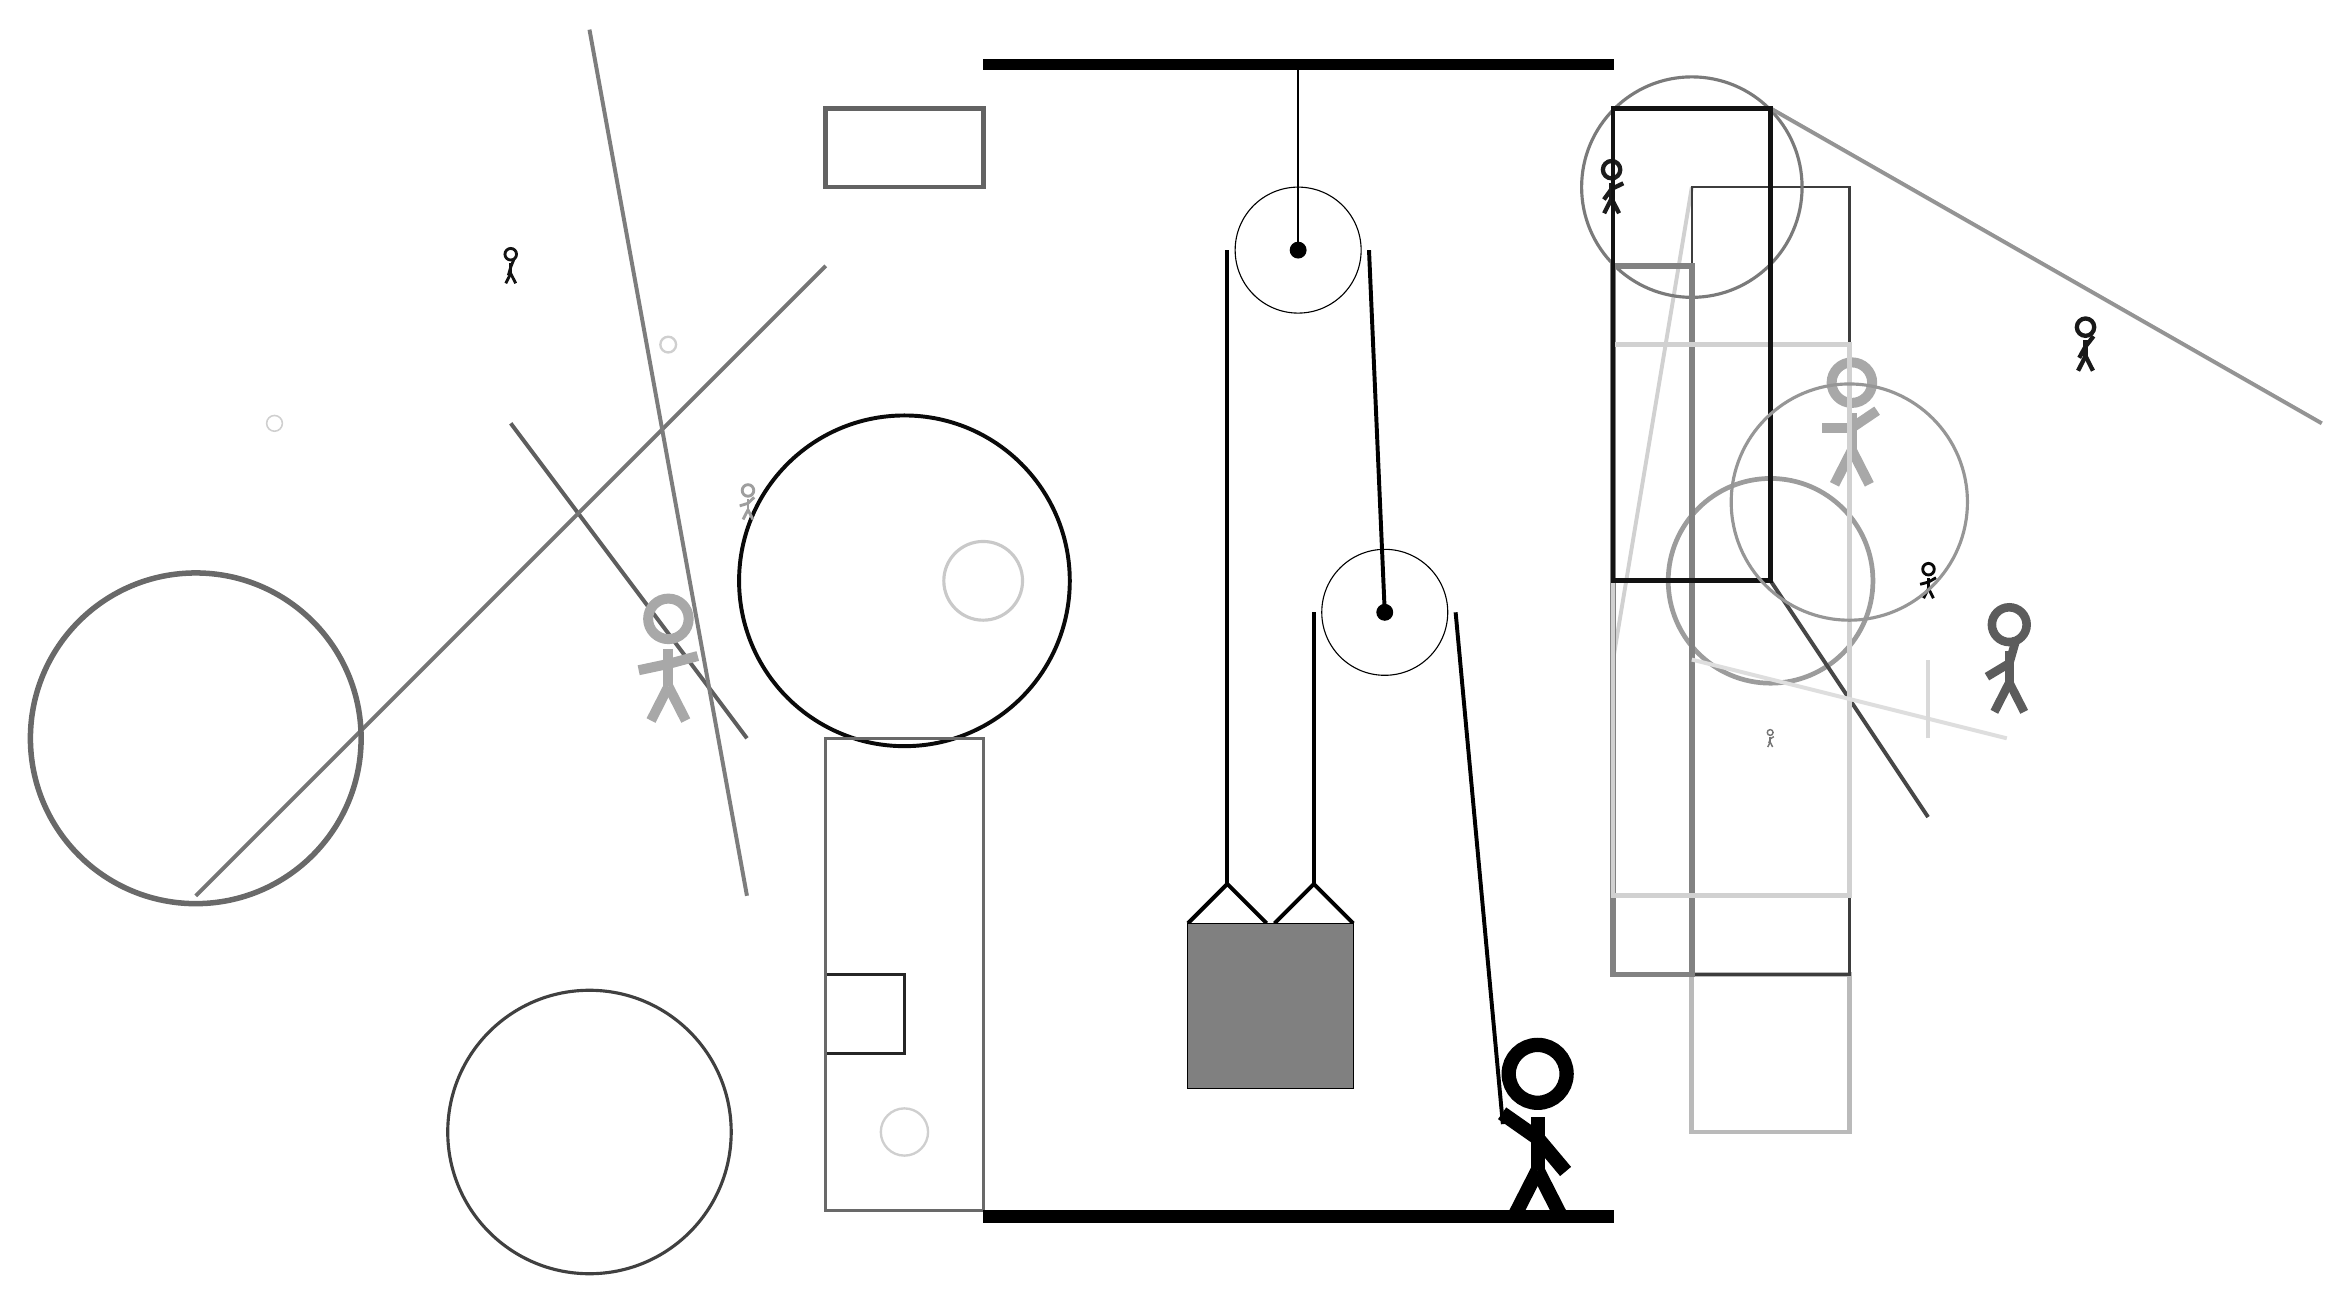
\begin{tikzpicture}
			%%%%% START %%%%%
			
			\draw[fill=black] (-2, 11.5) rectangle (6, 11.625);
			
			\draw (2, 9.2) circle (0.8);
			\draw[fill=black] (2, 9.2) circle (0.1);
			\draw[thick] (2, 9.2) -- (2, 11.5);
			
			\draw (3.1, 4.6) circle (0.8);
			\draw[fill=black] (3.1, 4.6) circle (0.1);
			
			\draw[line width = 0.5mm]  (0.6, 0.65) -- (1.1, 1.15) -- (1.6, 0.65);
			\draw[line width = 0.5mm]  (1.7, 0.65) -- (2.2, 1.15) -- (2.7, 0.65);
			\draw[fill=black!50] (0.6, 0.65) rectangle (2.7, -1.45);
			
			\draw[line width = 0.5mm] (1.1, 9.2) -- (1.1, 1.15);
			\centerarc[line width = 0.5mm](2, 9.2)(0:180:0.9);
			\draw[line width = 0.5mm] (2.9, 9.2) -- (3.1, 4.6);
			\draw[line width = 0.5mm] (2.2, 4.6) -- (2.2, 1.15);
			\centerarc[line width = 0.5mm](3.1, 4.6)(0:180:0.9);
			\draw[line width = 0.5mm] (4.0, 4.6) -- (4.6, -1.9);
			
			\node at (5, -2) {\Strichmaxerl[10][-35][-50]};
			
			\draw [line width=0.4mm, color=black!21](-2, 5) circle (0.5);
			
			\draw[line width=0.5mm, color=black!18](7, 10) -- (6, 4);
			\draw[line width=0.6mm, color=black!61] (-2, 10) rectangle (-4, 11);
			\draw [line width=0.3mm, color=black!19](-6, 8) circle (0.1);
			\draw [line width=0.6mm, color=black!39](8, 5) circle (1.3);
			
			\node[line width=0.5mm, color=black!93] at (-8, 9) {\Strichmaxerl[2][74][68]};
			\draw[line width=0.5mm, color=black!63](-5, 3) -- (-8, 7);
			\draw [line width=0.3mm, color=black!19](-3, -2) circle (0.3);
			\draw [line width=0.4mm, color=black!75](-7, -2) circle (1.8);
			\node[line width=0.3mm, color=black!34] at (-6, 4) {\Strichmaxerl[7][12][15]};
			\node[line width=0.2mm, color=black!64] at (11, 4) {\Strichmaxerl[6][31][74]};
			\draw[line width=0.4mm, color=black!85] (-4, 0) rectangle (-3, -1);
			\draw[line width=0.6mm, color=black!27] (7, 0) rectangle (9, -2);
			\node[line width=0.4mm, color=black!34] at (9, 7) {\Strichmaxerl[7][0][34]};
			\draw[line width=0.3mm, color=black!76] (7, 10) rectangle (9, 0);
			\draw [line width=0.5mm, color=black!96](-3, 5) circle (2.1);
			
			\node[line width=0.4mm, color=black!38] at (-5, 6) {\Strichmaxerl[2][17][44]};
			\draw[line width=0.5mm, color=black!54](-4, 9) -- (-12, 1);
			\draw [line width=0.7mm, color=black!59](-12, 3) circle (2.1);
			
			\draw [line width=0.4mm, color=black!52](7, 10) circle (1.4);
			\draw[line width=0.4mm, color=black!59] (-4, -3) rectangle (-2, 3);
			
			\draw[line width=0.7mm, color=black!49] (6, 9) rectangle (7, 0);
			
			\draw [line width=0.2mm, color=black!19](-11, 7) circle (0.1);
			\node[line width=0.5mm, color=black!97] at (10, 5) {\Strichmaxerl[2][15][30]};
			\draw[line width=0.5mm, color=black!72](10, 2) -- (8, 5);
			\node[line width=0.2mm, color=black!89] at (6, 10) {\Strichmaxerl[3][54][26]};
			\draw[line width=0.5mm, color=black!42](8, 11) -- (15, 7);
			\draw[line width=0.5mm, color=black!51](-5, 1) -- (-7, 12);
			\draw[line width=0.6mm, color=black!18] (6, 1) rectangle (9, 8);
			
			\draw[line width=0.5mm, color=black!13](11, 3) -- (7, 4);
			\node[line width=0.7mm, color=black!54] at (8, 3) {\Strichmaxerl[1][72][32]};
			
			\draw[line width=0.6mm, color=black!93] (8, 11) rectangle (6, 5);
			\node[line width=0.4mm, color=black!90] at (12, 8) {\Strichmaxerl[3][61][52]};
			\draw[line width=0.5mm, color=black!15](10, 3) -- (10, 4);
			\draw [line width=0.4mm, color=black!41](9, 6) circle (1.5);
			
			\draw[fill=black] (-2, -3) rectangle (6, -3.15);
			
			%%%%% END %%%%%
		\end{tikzpicture}
	\end{figure}	
\end{document}